\begin{multicols}{2}
	
%	\begin{minipage}{0.5\linewidth}
		
		\section{Fundamente}
			
			\textbf{Aufgaben}
			
				\begin{itemize}
					
					\item Bindeglied zwischen Bauwerk und Baugrund
					
					\item Sichere Lasteinleitung der Bauwerkslasten in den Baugrund
					
					\item  Bemessung, so dass keine Überschreitung
						\begin{itemize}
							
							\item der Tragfähigkeit des Bauteils und derjenigen des Bodens

							\item von zulässigen Setzungen, Verkippungen	
							
						\end{itemize}
					
					\item Boden-Bauwerks-Interaktion
					
					\item Aktivierung von Auflagerreaktionen erfordert Verformungen des Baugrunds
					
				\end{itemize}
		
		
%	\end{minipage}
%	\begin{minipage}{0.5\linewidth}
		
		\textbf{Arten}
		
		\begin{itemize}
			
			\item Flachgründungen (Einzel-, Streifen-, Plattenfundamente)
			
			\item Tiefgründungen (Pfahlfundationen, KPP)
			
			\item ggf. Zusatzmassnahmen (Baugrundverbesserung, Bodenersatz, …)
			
		\end{itemize}
		
		
%	\end{minipage}
%
%	\begin{minipage}{0.5\linewidth}
%		
		\subsection{Entwurfsregeln}
			
			\begin{enumerate}
				
				\item Abmessungen im Grundriss
					\begin{enumerate}
						
						\item Zulässige Bodenpressungen oder Sohldrücke: Annahme $ \sigma_{zul} $: zwischen 0.05 $ \frac{N}{mm^2} $ und 0.6 $ \frac{N}{mm^2} $ $\rightarrow$ abhängig von:
							\begin{itemize}
							
								\item Baugrundbeschaffenheit, Fundationstiefe, Topographie
								
								\item resultierenden Verformungen (Setzungen, Setzungsdifferenzen)
								
								\item lokalen Tragsicherheitsberechnungen
								
								\item Betrachtung der Gesamtstabilität (z.B. Kippen, Gleiten; Bauzustände)
																
							\end{itemize}
						
						\item Setzungen, Setzungsdifferenzen
							\begin{itemize}
								
								\item Berücksichtigung der Vorbelastung des Baugrundes durch Aushubmaterial
								
								\item benachbarte Fundamente möglichst gleiches
								Setzungsverhalten
								
							\end{itemize}
					
						\item Kippsicherheit und weiteres
							\begin{itemize}
								
								\item keine klaffende Fuge für ständige Lasten: Exzentrizität der Resultierenden innerhalb 1.
								Kernweite (= «Kern»): $ \frac{e_x}{b_x} + \frac{e_y}{b_y} \leq \frac{1}{6} $
								
								\item Begrenzung Exzentrizität innerhalb 2. Kernweite für
								ständige + veränderliche Lasten: Fundament soll bis
								zu seinem Schwerpunkt durch Druck belastet bleiben: $ \left( \frac{e_x}{b_x} \right)^2 + \left( \frac{e_y}{b_y} \right)^2 \leq \frac{1}{9} $
								
								\item Berücksichtigung exzentrischer Lastangriff Abschätzung Fundamentabmessung durch
								Reduktion der Fundamentfläche: $ A_{red} = ( a - 2 e_a) ( b - 2 e_b) $
								
							\end{itemize}
						
							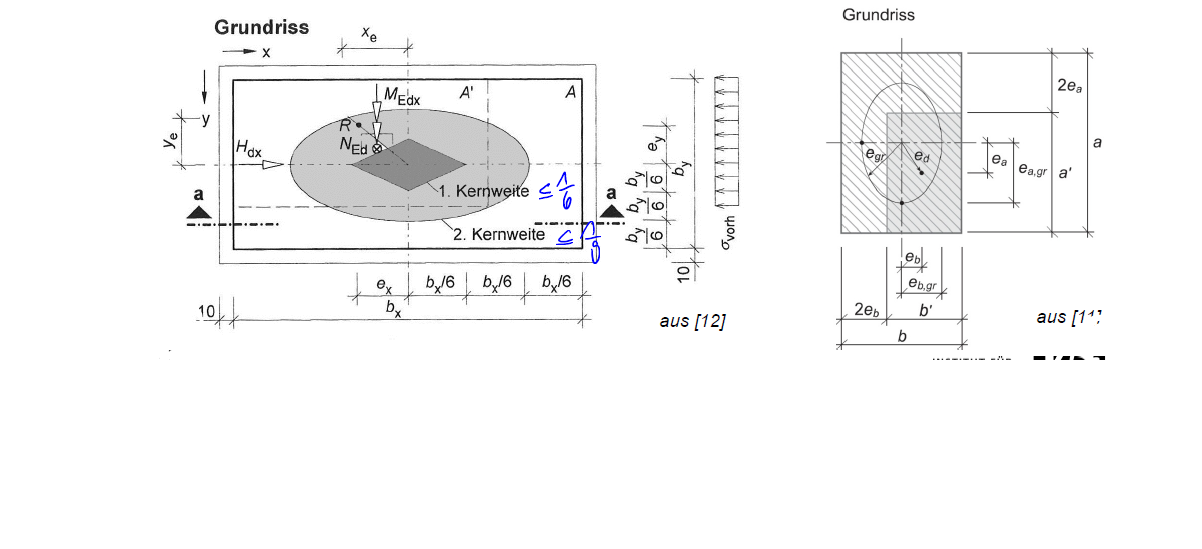
\includegraphics[width=2\linewidth, angle=270]{images/Fun1Kippsicherheit.PNG}
							
					\end{enumerate}
			
				\item Fundamentdicke
					\begin{enumerate}
					
						\item Mindestdicken (i.d.R. >200 bis 250mm)
							\begin{itemize}
								
								\item Einzelfundament: $ \frac{h_m}{b} \approx \frac{1}{4} \div \frac{1}{6} \geq h_{min}  $
								
								\item Streifenfundamente, Fundamentbalken: $ \frac{h_m}{l} \approx \frac{1}{8} \geq h_{min} $
								
								\item Plattenfundamente: $ \frac{h_m}{l} \approx \frac{1}{25} \div \frac{1}{30} \geq h_{min}  $
								
							\end{itemize}
					
						\item Anforderungen aus Biegung (meist bewehrt)
					
						\item Anforderungen aus Querkraft (Durchstanznachweis gem. Flachdecken)
					
					\end{enumerate}
			
				\item Fundamenttiefe
					\begin{itemize}
						
						\item Bodenbeschaffenheit (z.B. Tiefe der tragfähigen Schichten)
						\item Zulässige Bodenpressungen
						\item Setzungen
						\item Frosteindringtiefe: t $\geq$ 0.80m
						
						
					\end{itemize}
				
			\end{enumerate}
		
		
%	\end{minipage}
%	
%
%	\begin{minipage}{0.5\linewidth}
		
		\subsection{Bemessung}
			
			\begin{enumerate}
				
				\item Ermittlung der Sohldruckverteilung
				
				\item Biegebemessung
				
				\item Schubbemessung
				
				\item Konstruktive Durchbildung
				
			\end{enumerate}
		
		
		
%	\end{minipage}

\end{multicols}	

	\begin{minipage}{0.5\linewidth}
		
		
		
	\end{minipage}